\chapter{Introduction}
\section{Background}

Convolutional Neural Networks are widely used to achieve better accuracy in various deep learning and computer vision tasks. Since AlexNet won the 2012 ImageNet competition, CNNs (short for Convolutional Neural Networks) have become the de facto algorithms for a wide variety of tasks in deep learning, especially for computer vision. From 2012 to date, researchers have been experimenting and trying to come up with better and better architectures to improve models accuracy on different tasks. They are primarily developed on a fixed budget and scaled up to meet requirement later. The seminar details creation of efficient models as the competition is to beat the top accuracy; Scaling, if done correctly, can also help in improving the efficiency of a model.


\section{Definitions}

Here the topics are described and defined which are later required in the technical seminar.

\subsection{Convolutional Neural Networks (CNN)}

In deep learning, a convolutional neural network (CNN, or ConvNet) is a class of deep neural networks, most commonly applied to analyzing visual imagery. They are also known as shift invariant or space invariant artificial neural networks (SIANN), based on their shared-weights architecture and translation invariance characteristics. They have applications in image and video recognition, recommender systems, image classification, medical image analysis, natural language processing, and financial time series.

CNNs are regularized versions of multilayer perceptrons. Multilayer perceptrons usually mean fully connected networks, that is, each neuron in one layer is connected to all neurons in the next layer. The "fully-connectedness" of these networks makes them prone to overfitting data. Typical ways of regularization include adding some form of magnitude measurement of weights to the loss function. CNNs take a different approach towards regularization: they take advantage of the hierarchical pattern in data and assemble more complex patterns using smaller and simpler patterns. Therefore, on the scale of connectedness and complexity, CNNs are on the lower extreme.

Convolutional networks were inspired by biological processes in that the connectivity pattern between neurons resembles the organization of the animal visual cortex. Individual cortical neurons respond to stimuli only in a restricted region of the visual field known as the receptive field. The receptive fields of different neurons partially overlap such that they cover the entire visual field.
\begin{figure}[htpb]
\centering
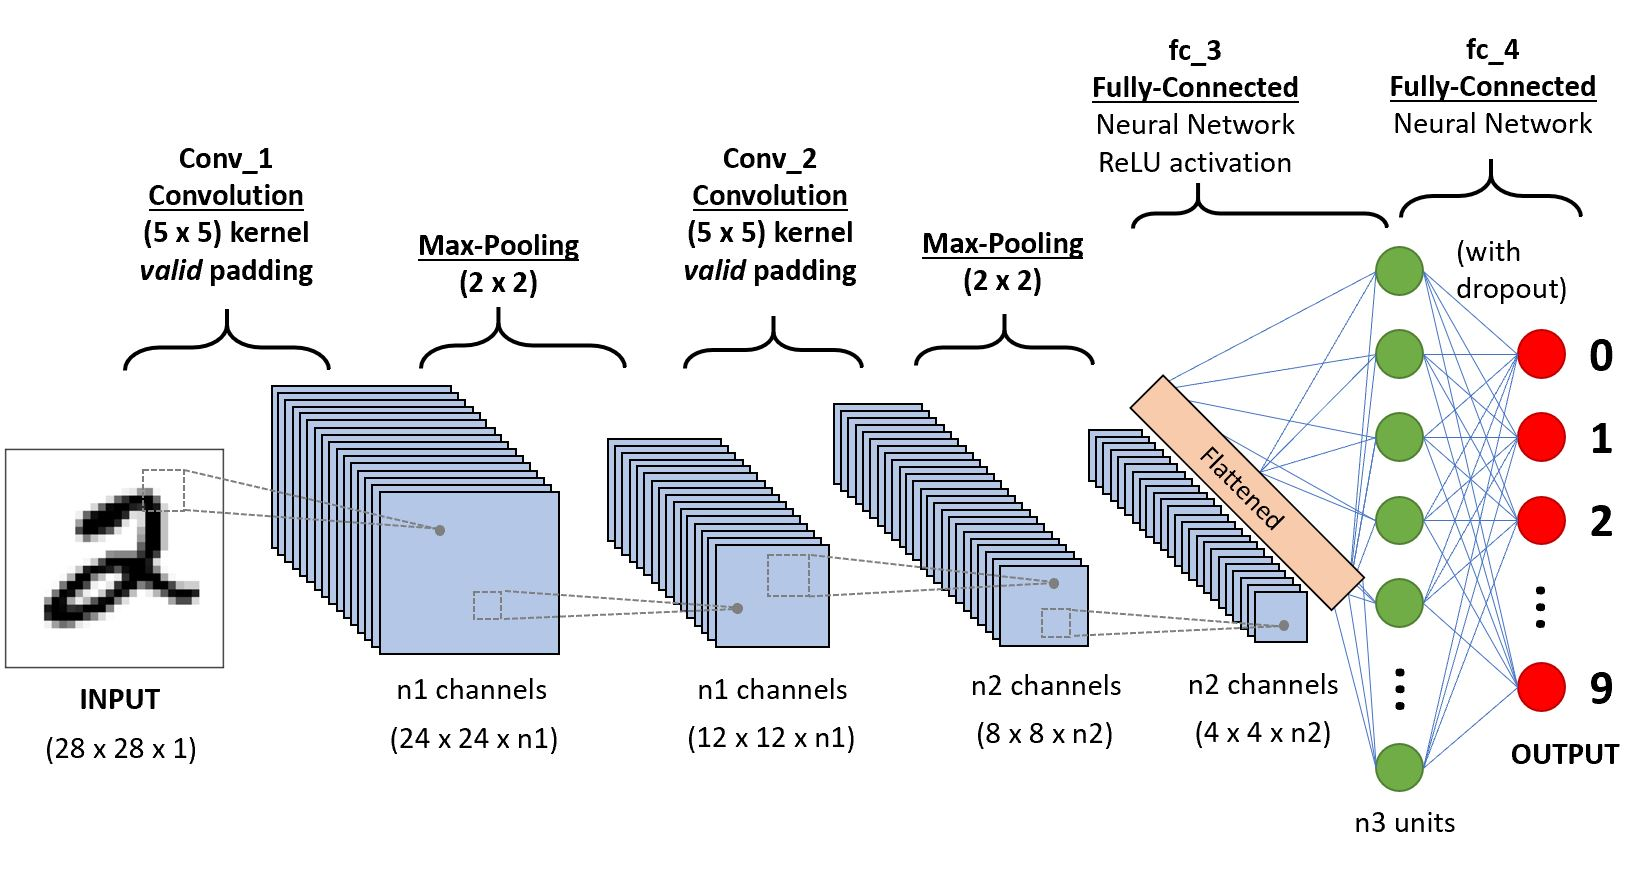
\includegraphics[width=\textwidth,height=\textheight,keepaspectratio]{../../static/ConvNet.jpg}
\caption{ConvNet.jpg}
\end{figure}
\subsection{Hyperparameters}

In machine learning, a hyperparameter is a parameter whose value is set before the learning process begins. By contrast, the values of other parameters are derived via training.

Hyperparameters can be classified as model hyperparameters, that cannot be inferred while fitting the machine to the training set because they refer to the model selection task, or algorithm hyperparameters, that in principle have no influence on the performance of the model but affect the speed and quality of the learning process. An example of a model hyperparameter is the topology and size of a neural network. Examples of algorithm hyperparameters are learning rate and mini-batch size.


\subsection{Grid Search}

The traditional way of performing hyperparameter optimization has been grid search, or a parameter sweep, which is simply an exhaustive searching through a manually specified subset of the hyperparameter space of a learning algorithm. A grid search algorithm must be guided by some performance metric, typically measured by cross-validation on the training set or evaluation on a held-out validation set.

Since the parameter space of a machine learner may include real-valued or unbounded value spaces for certain parameters, manually set bounds and discretization may be necessary before applying grid search.
\begin{figure}[htpb]
\centering
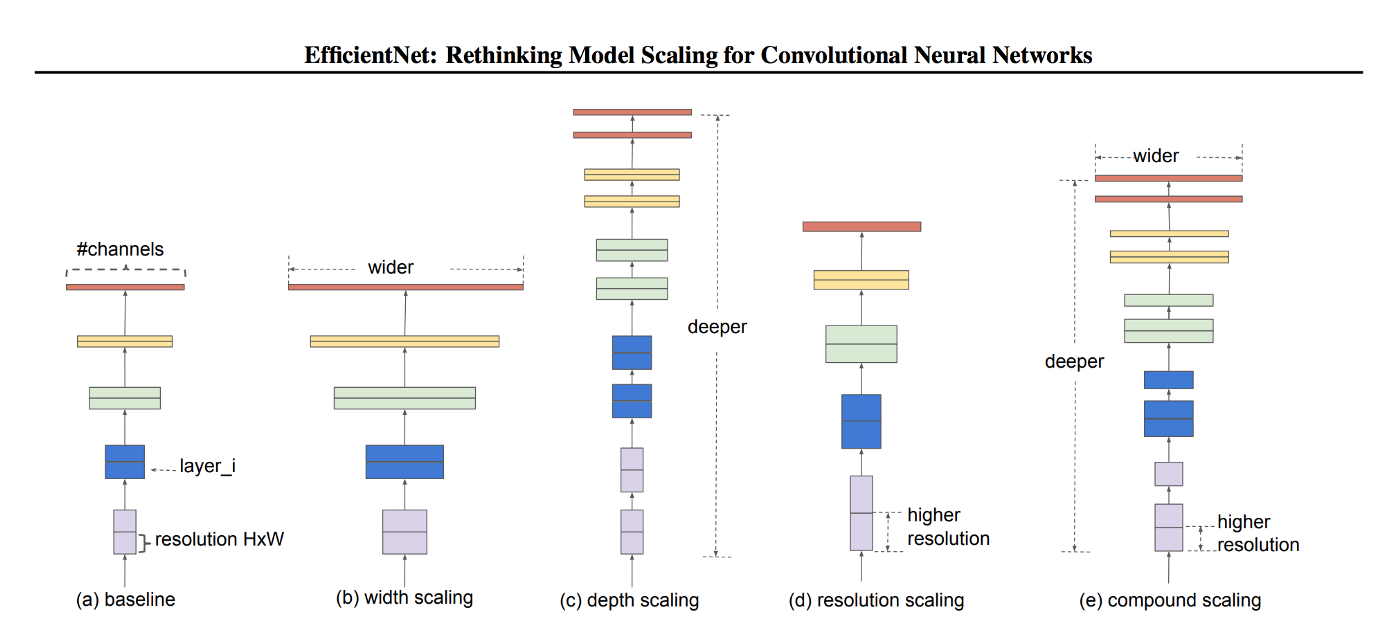
\includegraphics[width=\textwidth,height=\textheight,keepaspectratio]{../../static/Scaling parameters of CNN.png}
\caption{Scaling parameters of CNN.png}
\end{figure}
\subsection{Scaling}

There are three scaling dimensions of a CNN: depth, width, and resolution. Depth simply means how deep the networks is which is equivalent to the number of layers in it. Width simply means how wide the network is. One measure of width, for example, is the number of channels in a Conv layer whereas Resolution is simply the image resolution that is being passed to a CNN. Intuitively, the compound scaling method makes sense because if the input image is bigger, then the network needs more layers to increase the receptive field and more channels to capture more fine-grained patterns on the bigger image.